% !TEX root = ../agglo_clust_review.tex

\captionsetup[subfigure]{justification=centering, singlelinecheck=off}
\begin{figure}[t]
\centering
    \begin{subfigure}[t]{0.47 \textwidth}
        \centering
        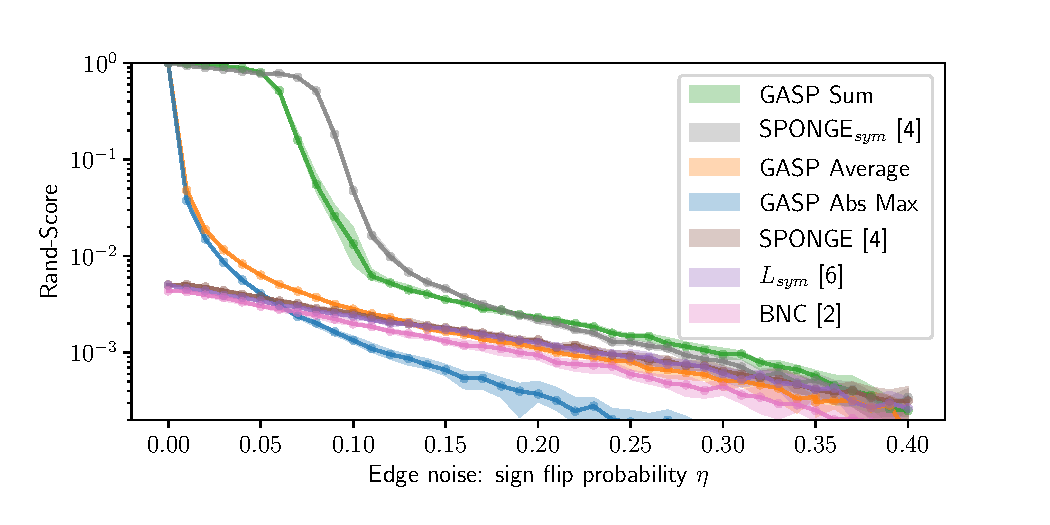
\includegraphics[width=\textwidth,trim=0.25in 0.in 0.5in 0.in,clip]{./figs/SSBM_experiments.pdf}
        \caption{Scores on SSBM graphs}
    \end{subfigure} \hfill
    \begin{subfigure}[t]{0.47 \textwidth}
        \centering
        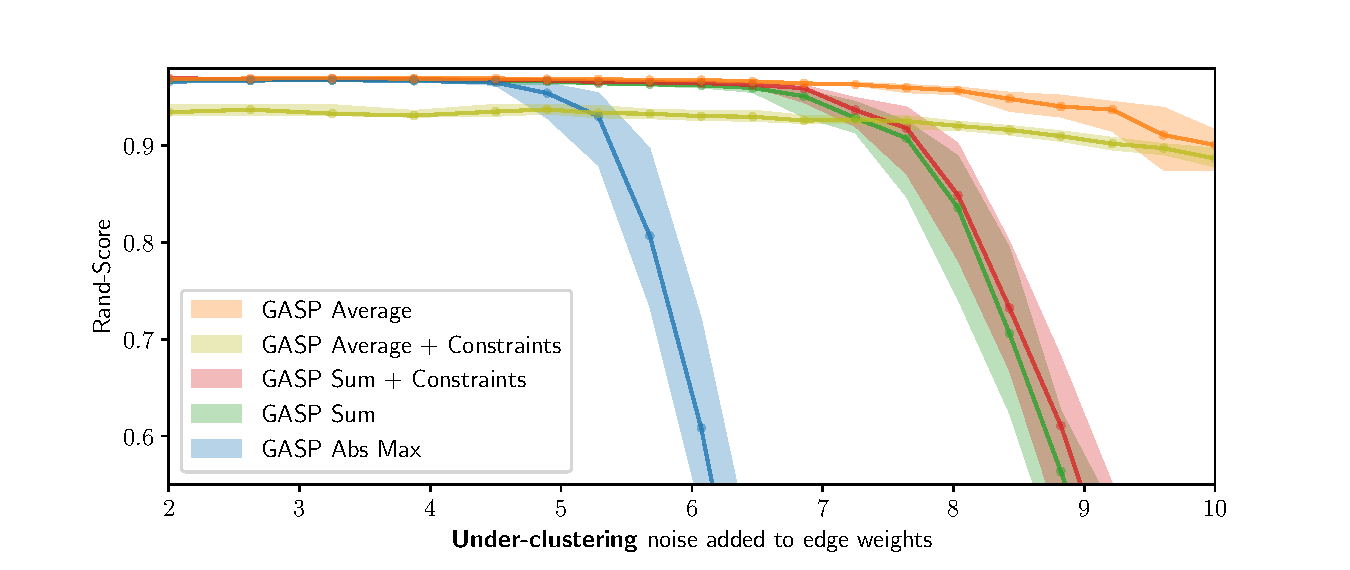
\includegraphics[width=\textwidth,trim=0.53in 0.1in 0.65in 0.45in,clip]{./figs/noise_plots/under_segment_plots_1.pdf}
        \caption{Scores on \emph{CREMI-gridGraph} perturbed with noise}
    \end{subfigure}

    % \begin{subfigure}[t]{0.32 \textwidth}
    %     \centering
    %     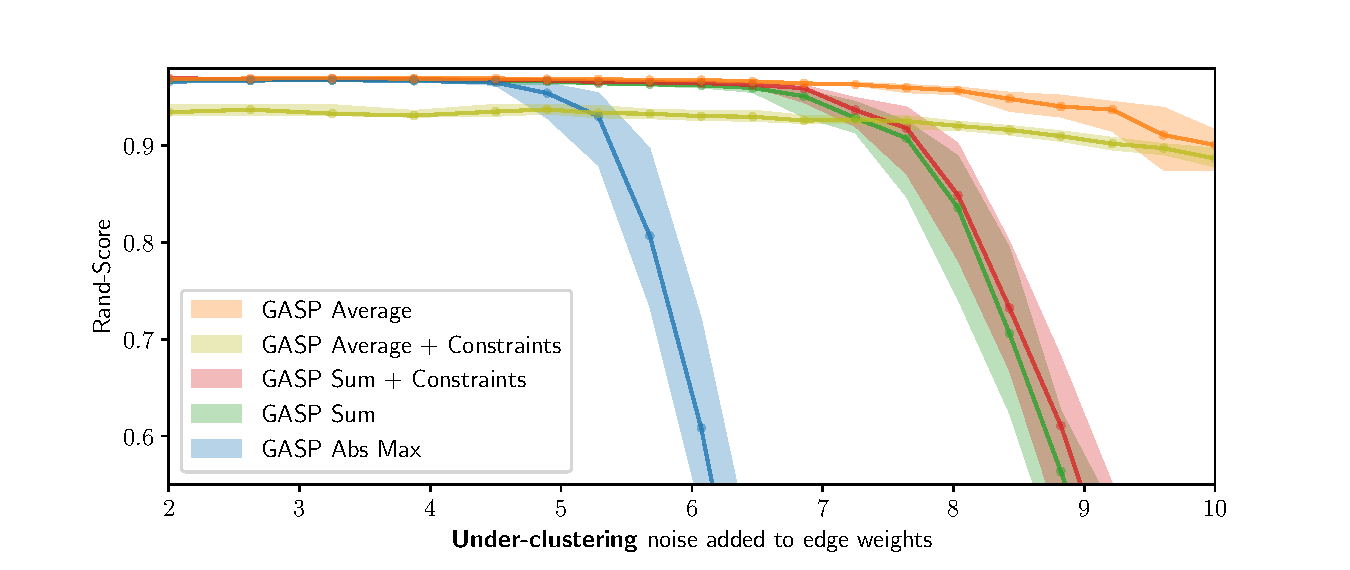
\includegraphics[width=\textwidth,trim=0.53in 0.1in 0.65in 0.45in,clip]{./figs/noise_plots/under_segment_plots_1.pdf}
    % \end{subfigure}\hfill
    % \begin{subfigure}[t]{0.32 \textwidth}
    %     \centering
    %     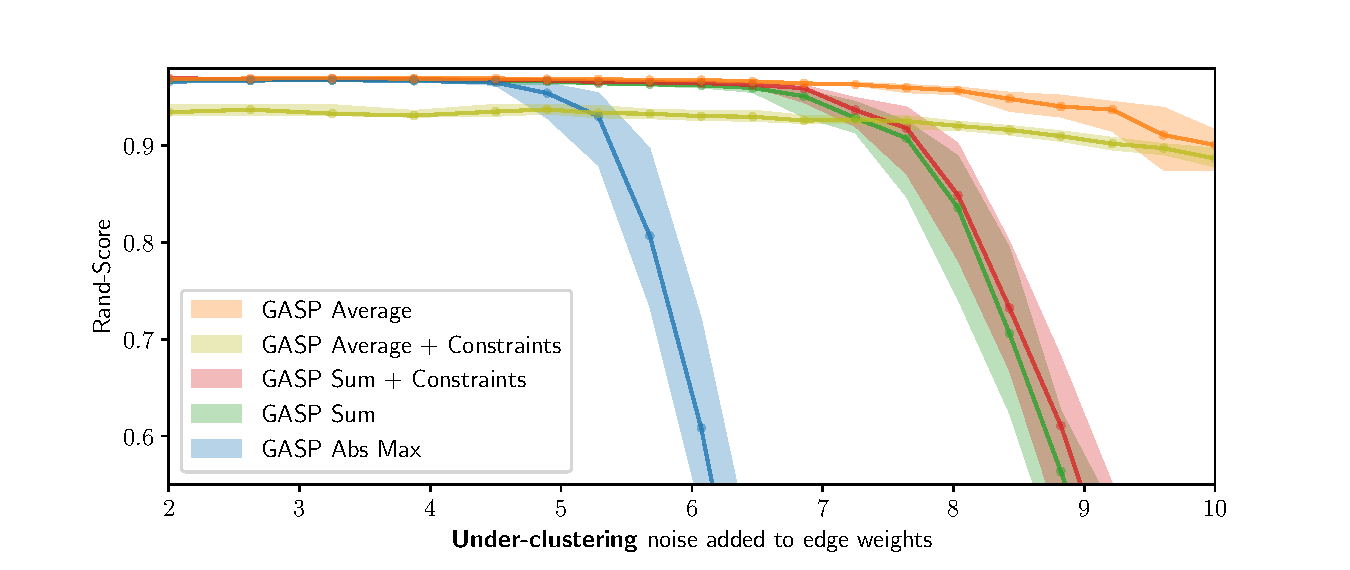
\includegraphics[width=\textwidth,trim=0.53in 0.1in 0.65in 0.45in,clip]{./figs/noise_plots/under_segment_plots_1.pdf}
    % \end{subfigure}
    %     \begin{subfigure}[t]{0.49 \textwidth}
    %     \centering
    %     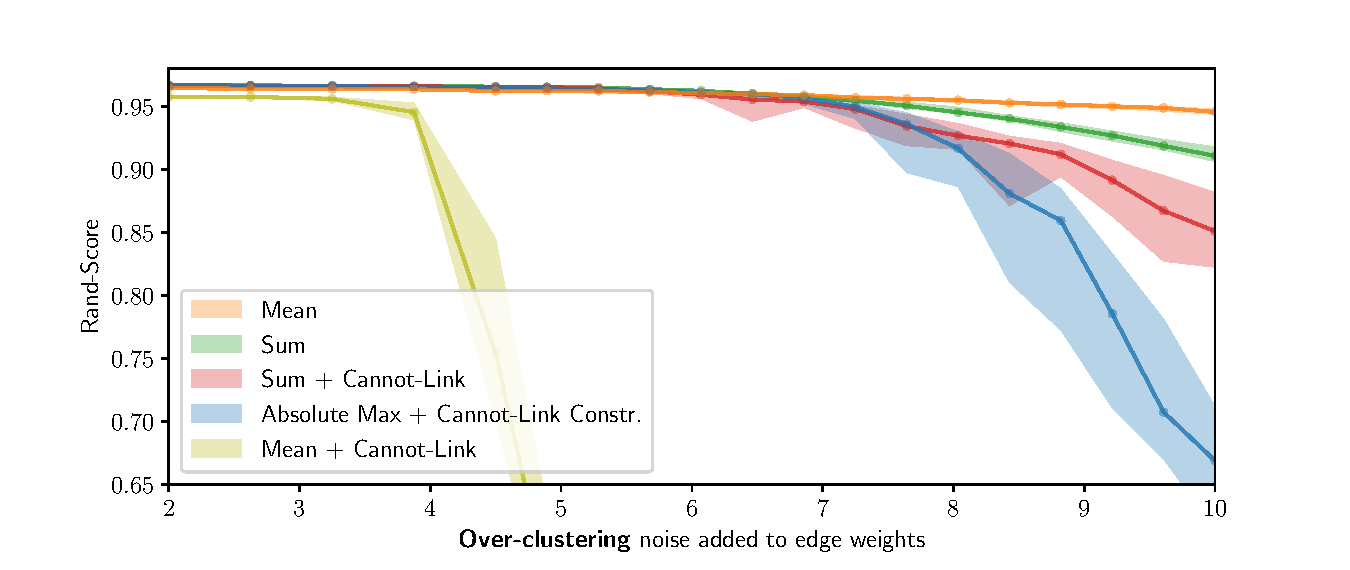
\includegraphics[width=\textwidth,trim=0.53in 0.1in 0.65in 0.45in,clip]{./figs/noise_plots/over_segment_plots_0.pdf}
    %     \caption{No long-range predictions: \\$p_{\mathrm{long}}=0$} \label{fig:merge_noise_only_direct}
    % \end{subfigure} \hfill
    % \begin{subfigure}[t]{0.49 \textwidth}
    %     \centering
    %     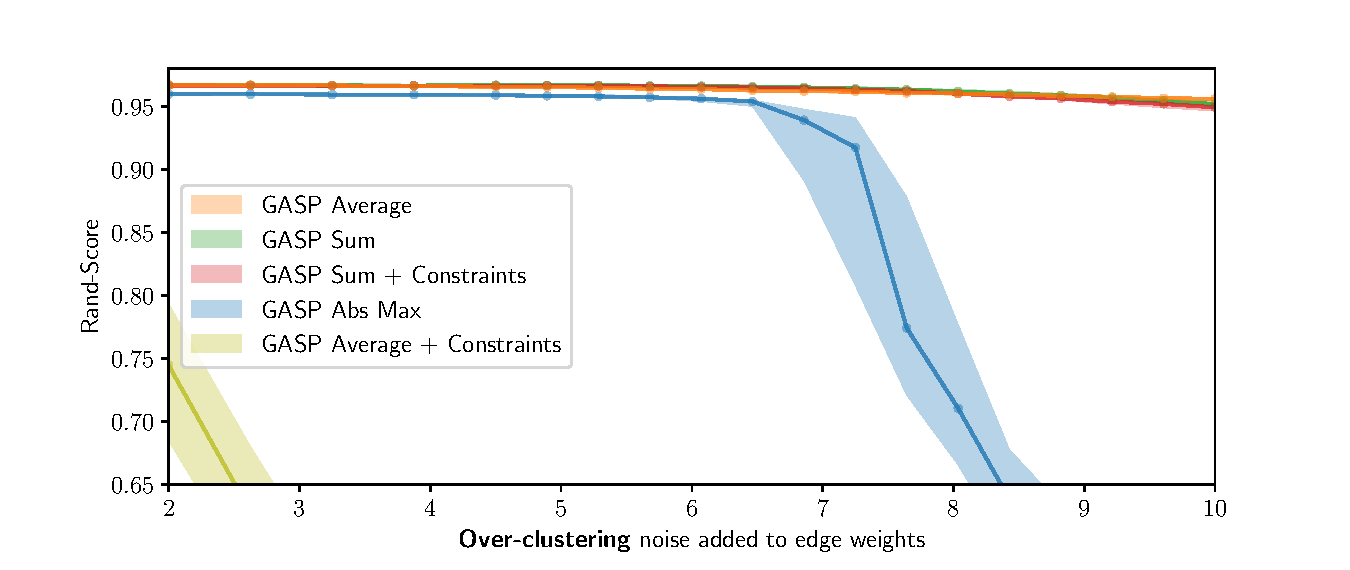
\includegraphics[width=\textwidth,trim=0.53in 0.1in 0.65in 0.45in,clip]{./figs/noise_plots/over_segment_plots_1.pdf}
    %     \caption{With long-range predictions: $p_{\mathrm{long}}=0.1$} \label{fig:merge_noise_with_long_range}
    % \end{subfigure}
\caption{\algname{} sensitivity to noise: \emph{Average} linkage proved to be the most robust. Performances are given by Rand-Score (higher is better) depending on the amount of noise added to the CNN predictions. Solid lines represent median values over 30 experiments. Values between the 25th and the 75th percentile are shown in shaded areas. The two sets of experiments using under- and over-clustering noise are summarized in the plots at the top and at the bottom, respectively (see Appendix \ref{sec:appendix_noise_gen} for more details). For each experiment, some of the long-range CNN predictions were randomly selected with probability $p_{\mathrm{long}}$ and added as long-range edges to the pixel grid-graph. Experiments are performed on a crop of CREMI training sample B.
\algname{} performances compared to spectral methods on synthetic graphs. The spectral methods were given the true number of clusters as input, in contrast to \algname{}. \TODO{Define paramters SSB; explain percentile stuff (for both noise experiments)}
}\label{fig:noise_plots}
\end{figure}


% \begin{figure}[t]
% \centering
% % \begin{minipage}[t]{0.48\textwidth}
% % \vspace{0pt}
% % \centering
% % % \footnotesize
% % \begin{tabular}[t]{L{9em} M{7em}}
% %            Method & Rand-Score \\ \midrule
% %            \textbf{GASP Average} & \textbf{0.8966} \\
% % GASP Sum & 0.8965 \\
% % GASP Abs Max & 0.8932 \\
% % SPONGE$_{sym}$ \cite{Cucuringu2019SPONGEAG} & 0.5839\\
% % $L_{sym}$ \cite{kunegis2010spectral} & 0.1931 \\
% % SPONGE \cite{Cucuringu2019SPONGEAG} & 0.0789 \\
% % BNC \cite{chiang2012scalable} & 0.0074 \\
% %         \end{tabular}
% %     \captionof{table}{\algname{} compared to spectral clustering methods on a small crop of the CREMI dataset (sample B).}
% %     \label{tab:cremi_spectral_experiments}
% % \end{minipage}\\\vspace{2em}
% \begin{minipage}[t]{0.38\textwidth}
% \vspace{0pt}
% \centering
%         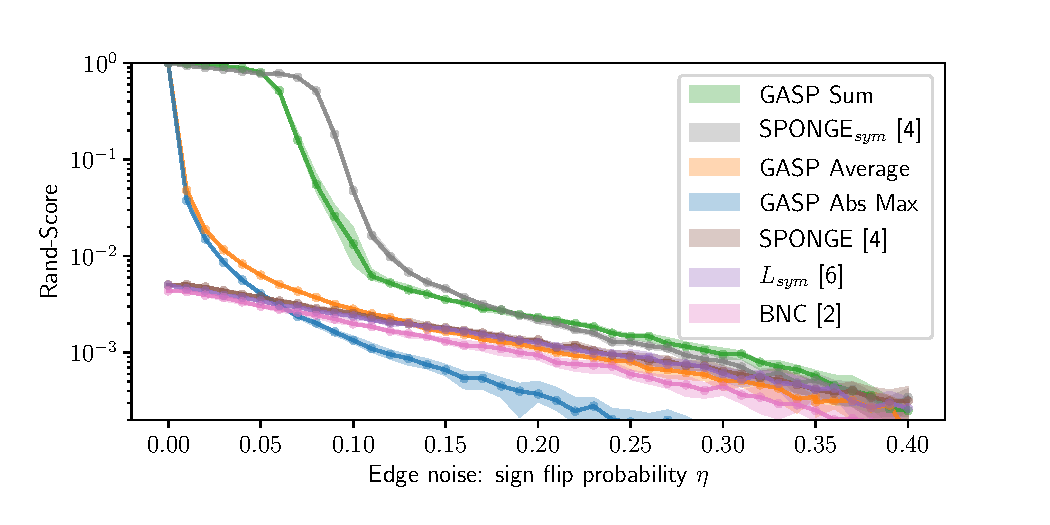
\includegraphics[width=1.\textwidth,trim=0.25in 0.25in 0.68in 0.36in,clip]{./figs/SSBM_experiments.pdf} % 0.45
%         \caption{}
%     \label{fig:SSBM_scores}
% \end{minipage}
% \end{figure}






% \subsection{Data: CREMI challenge} \label{sec:cremi_challenge}
% Test \ref{tab:cremi_leaderboard}
% We evaluate all algorithms in the proposed framework on the competitive CREMI 2016 EM Segmentation Challenge \cite{cremiChallenge} that is currently the neuron segmentation challenge with the largest amount of training data available. The dataset comes from serial section EM of \emph{Drosophila} fruit-fly tissue and consists of 6 volumes of 1250x1250x125 voxels at resolution 4x4x40nm, three of which come with publicly available training ground truth. The results submitted to the leaderboard are evaluated using the CREMI score, based on the Adapted Rand-Score (Rand-Score) and the Variation of Information Score \cite{arganda2015crowdsourcing}. In Appendix \ref{sec:cremi_details}, we provide more details about the training of our CNN model, inspired by work of \cite{lee2017superhuman,funke2018large}.
